\NeedsTeXFormat{LaTeX2e}
\documentclass[12pt]{article}

\usepackage{titlesec}
\usepackage{setspace}
\usepackage{amsmath}
\usepackage{amssymb}
\usepackage{epsfig}
\usepackage{fancybox}
\usepackage{listings}
%\usepackage{algo}
\usepackage{url}
\usepackage{xcolor}
\usepackage{adjustbox}
\usepackage{float}
\usepackage{multicol}
\usepackage[utf8]{inputenc}
\usepackage[colorlinks=true,linkcolor=blue]{hyperref}

\newcommand{\phil}[1]{{\color{red}(\textbf{Phil:} #1)}}
\newcommand{\yue}[1]{{\color{blue}(\textbf{Yue:} #1)}}
\newcommand{\specialcell}[2][c]{%
	\begin{tabular}[#1]{@{}c@{}}#2\end{tabular}}


\setlength{\textheight}{9in}
\setlength{\textwidth}{6in}
\setlength{\oddsidemargin}{.25in}
\setlength{\topmargin}{-.5in}  % changed from -.25 by RSR on 1/21/07
%\parindent .5in    % commented out by RSR 1/21/07

\hyphenation{itself}
\setcounter{secnumdepth}{4}
\setcounter{tocdepth}{4}
%%%%%
%% Commented out -- RSR, 1/21/07
%%%%%
% The following provides a box to surround the thesis statement
\newenvironment{Thesis}%
{\begin{Sbox}\begin{minipage}{.95\linewidth}}%
		{\end{minipage}\end{Sbox}\begin{center}\fbox{\TheSbox}\end{center}}

\title{Stream Mining Algorithms for Sensor Data Classification}
\author{
    Yue Dong\\
	\texttt{yuedong029@uottawa.ca}
	\and
	Philippe Paradis\\
	\texttt{philippe.paradis@carleton.ca}
}

\begin{document}
\singlespace
\maketitle

\tableofcontents
\newpage
\section*{Acknowledgements}


\begin{abstract}                % ~350 words max


\end{abstract}

% This sets section-numbering to only include Section and Subsection numbers
\setcounter{secnumdepth}{4}

\section{Introduction}
\label{sec:introduction}

\section{Dataset \& Data exploration}
\subsection{Dataset}
The dataset we used is the Bike Sharing Dataset from the UCI repository. Ac coding to the dataset description, ``this dataset contains the hourly and daily count of rental bikes between years 2011 and 2012 in Capital bikeshare system with the corresponding weather and seasonal information.''
 The summary of this dataset is as Table \ref{table:dataset} shows. More information of the dataset can be found at \url{http://archive.ics.uci.edu/ml/datasets/Bike+Sharing+Dataset}.
 
 \begin{table}[H]
 	\label{table:dataset}
 	\begin{tabular}{| l | p{11cm} |} \hline
 		Number of instances: & 17389 (hours), 731 (days)\\
 		Number of Attributes: & 16\\ \hline \hline
 		\textbf{Attributes details:} &\\ \hline
 		Attribute name  & description\\ \hline
 		instant   & record index\\ \hline
 		dteday    & date\\ \hline
 		season  & season (1:springer, 2:summer, 3:fall, 4:winter)\\ \hline
 		yr    &  year (0: 2011, 1:2012)\\ \hline
 		mnth &   month ( 1 to 12)\\ \hline
 		hr & hour (0 to 23) \\ \hline
 		holiday   & weather day is holiday or not \\ \hline
 		weekday   &  day of the week \\ \hline
 		workingday   & 1: if day is neither weekend nor holiday; 0: otherwise.\\ \hline
 		weathersit   & 1: Clear; 2: Mist; 3: Light Snow, Light Rain; 4: Heavy Rain, Ice Pallets, Snow + Fog;\\ \hline
 		temp   & Normalized temperature in Celsius. \\ \hline
 		atemp    & Normalized feeling temperature in Celsius. \\ \hline
 		windspeed   & Normalized wind speed. \\ \hline
 		casual   & count of casual users\\ \hline
 		registered   & count of registered users\\ \hline
 		cnt   & count of total rental bikes including both casual and registered \\ \hline
 	\end{tabular}
 	\caption{Bike sharing dataset summary}
 \end{table}
\subsection{Data Visualization}
\label{sec:visual}

\begin{figure}[H]
	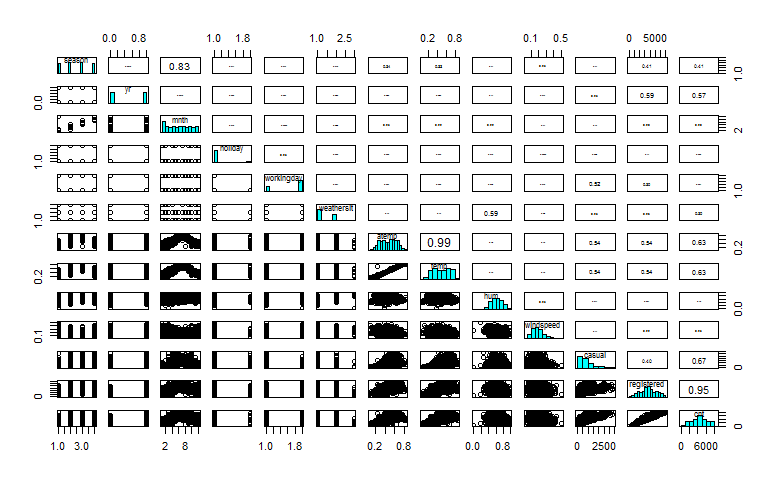
\includegraphics[scale=0.6]{figures/scatterplot.png}
	\label{fig:scatterplot}
	\caption{Scatterplot matrix of bike sharing (daily) dataset}
\end{figure}

As we can see from Figure \ref{fig:scatterplot}, there are 0.83 correlation between season and mnth, 0.99 correlation between temp and atemp, and 0.95 correlation between registered and cnt, 0.67 between casual and cnt.

High correlation between two variables means that as one variable rises or falls, the other variable rises or falls as well. Since we don't want high correlation in our dataset, we can drop month, and atemp.

Moreover, from observing the last three columns of correlation between different attributes to registered, casual, and cnt, we can have a list of the correlations in decreasing order as the following table shows: 
\begin{table}[H]
	\begin{tabular}{| l | l | l | l | l | l|}
		cnt~ & registered & casual & temp/atemp & yr & season\\
		correlation & 0.95 & 0.67 & 0.63 & 0.57 & 0.41\\
		\hline
	%	registered~ &
	\end{tabular}
\end{table}
Random sampling 1000 instances without replacement, and draw the scatterplot matrix shows that the hours have a high correlation with the hourly cnt. 
\begin{figure}[H]
	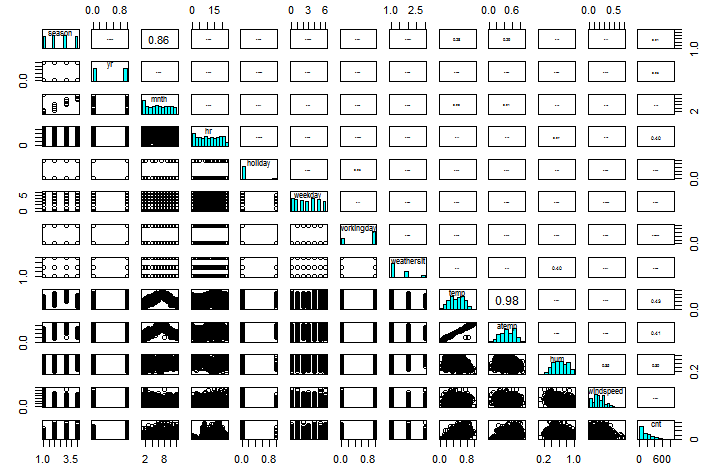
\includegraphics[scale=0.8]{figures/scatterplot_col_season.png}
	\end{figure}

Therefore, we identify that temp, yr, season/mth, hr, and workingday as our main focus.

1. Most likely, temperature and weather have correlation with bike demand. We can plot:

Explore 2. Most certain the hour of the day also correlates with Bike demand 

Explore 3. Finally let’s see if usage varies depending on the month 

In short we have identified strong correlation with these predictors: 1. Temperature 2. Hour of the Day 3. Working Day 4. Month of the Year

\subsection{Association Rule Mining}
From the data visualization, there is one unanswered question left: How can we know where the PEAK rental periods are on an overall basis?

To find more about this, we did an association rule mining. The bike sharing dataset contains a mixture of categorical and numeric attributes and therefore need some preparation before using apriori algorithm on it.

temp : Normalized temperature in Celsius. The values are divided to 41 (max)
- atemp: Normalized feeling temperature in Celsius. The values are divided to 50 (max)
- hum: Normalized humidity. The values are divided to 100 (max)
- windspeed: Normalized wind speed. The values are divided to 67 (max)

\section{Unsupervised Learning: Data Preprocessing}
\subsection{Dimension Reduction: PCA }
\label{sec:dimension-reduction}

\subsection{Data Reduction: Clustering kmeans+Davies-Bouldi index}
\label{data-reduction}

The bike sharing dataset has  17365 data instances for the hourly bike sharing dataset. Instead of dimension reduction to reduce the number of attributes, we can use data reduction to reduce the number of cases. In this section, we consider to use clustering methods to cluster together similar cases and also try unsupervised learning for outlier detection. By doing so, we can have a reduced representation in volume but produces the same or similar analytical results.
\subsubsection{Fill in missing values}
Data cleaning, smooth noisy data, identify or remove outliers, and resolve inconsistencies
\subsubsection{Data transformation}

\subsection{Data Reduction: Outlier Detection}






\section{Experimental Design}
\label{sec:experimental-design}



\subsection{Supervised Learning}
\label{supervised learning}


\section{Experiments and Results}
\label{sec:experiments-and-results}

\section{Kaggle}


\section{Conclusion and Further Work}
\label{sec:conclusion}



\begin{thebibliography}{9}
\bibitem{dataset}
Fanaee-T, Hadi, and Gama, Joao, 'Event labeling combining ensemble detectors and background knowledge', Progress in Artificial Intelligence (2013): pp. 1-15, Springer Berlin Heidelberg.
\end{thebibliography}

\end{document}
